
To precisely define what behavior the \openshmem interface guarantees for both users and
    implementers, this section formally defines an API-level memory model. An API-level
    model builds upon a programming language-level (PL-level) memory model, and it
    defines how API operations impact memory. This is useful for determining the
    ordering and visibility requirements for \openshmem memory accesses when implemented
    on any device, but it is of particular importance for devices like GPUs that have
    software managed caches requiring expensive bulk flush or invalidate actions to
    enforce memory ordering guarantees. Without a precisely specified memory model, API
    implementers and users may disagree on what behavior is guaranteed by the API, and
    this can lead to poor performance (too many bulk cache actions) or buggy code (too
    few bulk cache actions).

This section describes how \openshmem extends the C11 memory consistency model. C11 is
    used as the reference programming-language memory model because it underlies the
    rest of this specification. The API-level guarantees defined here are normative for
    \openshmem implementations regardless of the programming-language memory model used
    by an implementation. Section~\ref{subsubsec:api_pl_baseline} summarizes the
    baseline C11 memory model,
    Sections~\ref{subsubsec:api_model_overview}-\ref{subsubsec:api_integrate} describe
    how this programming-language model is extended to provide API-level semantics for
    \openshmem, and Section~\ref{subsubsec:api_scoped} describes how the guarantees of
    the API-level model can be adapted for GPU memory models.

\subsubsection{Baseline PL-level Axiomatic Memory Model (C11)}\label{subsubsec:api_pl_baseline}

A memory consistency model (MCM) specifies the executions that are permitted in a
    multithreaded program, including the values that read operations may return. One
    common way to formalize an MCM is through axioms over relations among events in an
    execution graph. Axiomatic formalization begins by considering candidate executions
    of a parallel program. In a candidate execution, each read is associated with a
    write to the same memory location—including the initial write to that location—from
    which it obtains its value. The model then defines relations among the events in
    these candidate executions and uses axioms over those relations to determine which
    executions are legal. These constraints limit the reorderings allowed by the
    compilers and hardware.

The C11 memory model is defined axiomatically in the C11 specification \S5.1.2.4.
    Although many prior works aim to mathematize or improve this formalism, the intent
    here is simply to provide sufficient understanding to build upon it with the
    \openshmem API model.

Under the PL-level C11 memory model, events consist of reads (\EVENT{R}), writes
    (\EVENT{W}), atomic read-modify-writes (\EVENT{RMW}, which perform both a read and
    write to memory), and fences (\EVENT{F}). Events that access memory may be atomic or
    non-atomic. Atomic events are associated with a memory order which can be acquire,
    release, acquire-release, or relaxed. These memory orders determine how atomic
    accesses can legally synchronize (release and acquire are used with the source and
    destination of a synchronizing access pair, respectively). The following relations
    are defined over the events in a candidate execution, and will be used to derive
    API-level relations in Section~\ref{subsubsec:api_relations}:

\begin{itemize}
    \item \textbf{Sequenced before (\REL{sb}):} Relates memory events from the same
        thread based on the order they are evaluated (also called program order in some
        contexts)
    \item \textbf{Modification order (\REL{mo}):} A total ordering between all modifying
        accesses (writes or read-modify-writes) to the same memory location.
    \item \textbf{Reads-from (\REL{rf}):} Relates a write \EVENT{W} and any read
        \EVENT{R} to the same memory location such that \EVENT{R} returns the value
        written by \EVENT{W}.
    \item \textbf{Synchronizes-with (\REL{sw}):} Same as \REL{rf}, but also requires
        that \EVENT{W} and \EVENT{R} are atomic, \EVENT{W} has release or
        acquire-release memory order, and \EVENT{R} has acquire or acquire-release
        memory order (this relation is also called synchronization order in some
        contexts).
    \item \textbf{Happens-before (\REL{hb}):} Transitive closure of \relSW{} and
        \relSB{}.
\end{itemize}

Furthermore, a \textbf{data race} is defined as a relation between two accesses $A$ and
    $B$ where all of the following are true:
\begin{itemize}
    \item $A$ and $B$ access the same memory location.
    \item At least one access is a modifying access (write or read-modify-write).
    \item At least one access is not atomic.
    \item $A$ and $B$ are not related by \relHB{}.
\end{itemize}

Although the axiomatic model places no requirements on when each event must update or
    access physical memory, it prohibits executions that don't adhere to a set of
    constraints, and by extension it disallows any architecture or compilation scheme
    that can result in such an execution. Specifically, C11 constrains candidate
    execution with the following axioms:

\begin{itemize}
    \item $acyclic(hb)$: \relHB{} cannot have any cycles.
    \item $irreflexive(rf;hb)$: \relHB{} must be consistent with the \relRF{} relation.
    \item $irreflexive((rf^{-1})^{?};mo;rf^?;hb)$: \relHB{} must be consistent with
        \relMO{} between writes, and it must also be consistent with the order of reads
        that read from writes in \relMO{} (often called coherence requirement).
    \item $irreflexive(rf \cup (mo;mo;rf^{-1}) \cup (mo;rf))$: The read of an atomic
        read-modify-write access must always read the last value (in \relMO{}) written
        before the write of the read-modify-write access (often called RMW atomicity).
\end{itemize}

Finally, the C11 specification states that, if a data race exists in a candidate
    execution that satisfies the above axioms, then the program's behavior is undefined.
    If a data race does not exist, then the program's behavior must conform to one of
    the conforming candidate executions.

\begin{description}
\apinotes{Consume and sequentially consistent memory orders are omitted from the above
    formalism for simplicity, so the baseline summarized here is a subset of the full
    C11 model. Language-level atomic accesses, including sequentially consistent
    accesses, are treated as ordinary accesses by the API-level model and do not by
    themselves synchronize with \openshmem operations. Accesses to the same location by
    a language-level atomic and an \openshmem operation must be ordered by \relAHB{} to
    avoid an API data race (Section~\ref{subsubsec:api_integrate}).
Also, instead of the verbose prose axioms defined in the C11 specification, the C11
    axioms are expressed above using the more concise (and equivalent) representation
    outlined by Batty et al. in "Overhauling SC atomics in C11 and OpenCL" (Symposium on
    the Principles of Programming Languages, 2016).}
\end{description}


\subsubsection{API-Level Memory Model Overview}\label{subsubsec:api_model_overview}

The \openshmem API-level memory model extends the C11 memory consistency model to define
    how \openshmem operations interact with memory. C11 is the reference model for this
    formalization; the resulting API-level guarantees apply regardless of the
    programming-language memory model used by an implementation. PL-level models use
    acquire and release semantics to establish ordering relations between fine-grain
    reads, writes, and fences. The API-level model additionally specifies ordering for
    coarse-grain operations such as \GET{}, \PUT{}, and barriers, which can execute
    asynchronously and involve multiple \acp{PE}.
The API-level model captures these higher-level ordering requirements by defining
    operation events and API-level ordering relations. An implementation may lower these
    relations to PL-level operations and relations, enabling different backend
    implementations while preserving the API-level guarantees.

To describe the desired \openshmem behavior, the API-level memory model makes the
    following additions to the existing PL-level model:

\begin{enumerate}
	\item\label{mcmsteps:one} \textbf{\acp{PE} and operation events}:
	    Section~\ref{subsubsec:api_pes_operations} introduces a new event type that
	    corresponds to an API operation and a new memory location property that specifies
	    the target \ac{PE}. This provides a basis for operation-level semantics across
	    multiple \ac{PE} memories.
	\item\label{mcmsteps:two} \textbf{Per-operation observable accesses}: For each
	    operation type, Section~\ref{subsubsec:api_observable} defines the minimum set of
	    observable memory accesses entailed by that operation. These accesses are not
	    related to the initiating thread by \relSB{}, which allows the thread to continue
	    execution while observable accesses execute asynchronously.
	\item\label{mcmsteps:four} \textbf{Coalesced collectives}:
	    Section~\ref{subsubsec:api_fused} coalesces matched collective operation calls into
	    a single event. This supports multi-PE collective operations and establishes
	    ordering across \acp{PE} even when there are no observable accesses.
	\item\label{mcmsteps:three} \textbf{API-level relations}:
	    Section~\ref{subsubsec:api_relations} defines new API-level ordering relations over
	    operation events and their observable accesses that will constrain \openshmem
	    memory ordering. This allows the programmer to explicitly enforce ordering of
	    asynchronous operations using the ordering and synchronization operations provided
	    by \openshmem. These relations are illustrated in
	    Section~\ref{subsubsec:api_relations_example}.
	\item\label{mcmsteps:five} \textbf{Updated relations, axioms}:
	    Section~\ref{subsubsec:api_integrate} updates the PL-level memory model axioms to
	    incorporate these new events and relations. By extending existing relations and
	    axioms (e.g., \relHB{}, data races) for the API level, we establish a memory model
	    that formalizes \openshmem ordering requirements.
\end{enumerate}

After defining how \openshmem extends the C11 memory model,
    Section~\ref{subsubsec:api_scoped} describes how the addition of scoped
    synchronization in GPU memory models impacts the API-level model.

\subsubsection{PEs and Operation Events}\label{subsubsec:api_pes_operations}

When defining behavior at the \openshmem API level, there are two key differences in
    program representation relative to a PL-level program.
\begin{enumerate}
    \item Applications span multiple \acp{PE}, each of which has its own memory space.
        Therefore, the PL-level definition of memory location and memory conflicts is
        extended to include both the memory address and the target \ac{PE} ID of a
        memory access.
    \item \openshmem operations are modeled as a distinct kind of event in the API memory
        model: an operation event. Each operation event has a specified type, and each
        type defines a set of minimum observable accesses that the operation entails, as
        described below. Operation events participate in \relSB{} and in relations
        derived from \relSB{}, alongside ordinary thread-access events. However,
        operation events do not themselves participate directly in access-based relations
        such as \relMO{}, \relRF{}, and \relSW{}; the observable accesses associated with
        an operation event may participate in those relations.
\end{enumerate}

The \ac{PE} ID of an observable access generated by an operation event (an ``observable
    access'') is defined in Table~\ref{table:api_observable} as either the \ac{PE} of
    the calling thread (\texttt{my\_pe}) or a \ac{PE} ID provided as a parameter to the
    operation.
A PL-level read, write, or RMW access is called an ``ordinary access.'' Its \ac{PE} ID
    is the \ac{PE} of the calling thread, unless its address is derived from a
    \FUNC{shmem\_ptr} operation, in which case its \ac{PE} ID is the target \ac{PE}
    specified by that operation.

\subsubsection{Per-Operation Observable Accesses}\label{subsubsec:api_observable}

For the purposes of the API memory model, each \openshmem operation type defines a
    minimum set of observable memory accesses that the operation must perform. These
    accesses are ``issued'' by the associated operation and must occur as part of it.
    The model does not constrain which thread executes an observable access; it may be
    executed by the initiating thread or another thread. An implementation may also
    perform other accesses for internal purposes, such as synchronization or buffering,
    but data accessed solely for those purposes must not be accessed by code outside the
    implementation.
Observable accesses have the same semantics as ordinary accesses and participate in the
    same access-based relations, with two exceptions:
\begin{enumerate}
  \item There is no \relSB{} ordering between a thread calling an \openshmem operation
      and observable accesses issued by that operation. The operation event itself is
      \relSB{} ordered with events in the calling thread, but this alone does not
      constrain the observable accesses. Instead, the API-level relations in
      Section~\ref{subsubsec:api_relations} define their ordering.
  \item Observable accesses do not have API-level atomic, acquire, or release semantics.
      An implementation may lower them to PL-level accesses with such semantics, but
      API-level ordering and data-race conditions are defined in terms of the issuing
      operation (Sections~\ref{subsubsec:api_relations}
      and~\ref{subsubsec:api_integrate}).
\end{enumerate}
%In addition, accesses performed by an implementation that are not included in the observable set must not modify data that may be observed from application code external to \openshmem operation implementations. 

Table~\ref{table:api_observable} defines the observable accesses performed for each
    \openshmem operation. Each access denotes the memory location as well as the \ac{PE}
    it targets ($my\_pe$ refers to the \ac{PE} of the initiating thread).
In many cases, control and compute pseudocode are included to define which memory
    locations are accessed, which values are written, and which values must eventually be
    read (pseudocode rather than C11 is used here because it allows clearer
    specification of where memory accesses are required).
However, this single-threaded control flow does not constrain the actual implementation
    and does not necessarily imply a total \relSB{} ordering between observable
    accesses. Within an operation, \relSB{} is defined to exist only between observable
    accesses when there is a true control or data dependency between two accesses (i.e.,
    no \relSB{} relation across independent iterations of a loop).
Specifically, $(A, B) \in sb$ only if $A$ and $B$ are observable accesses issued by the
    same operation and one of the following is true:
    \begin{itemize}
        \item $B$ takes a value derived from $A$ as an operand.
        \item $B$ has a control dependency on the result of $A$ such that $A$'s
            evaluation determines whether $B$ will occur.
	\item $B$ has an ordering dependency on $A$. This type of dependency currently exists
	    only in blocking and non-blocking \emph{put-with-signal} operations where the final
	    write to $sig\_addr$ is ordered after all prior observable accesses to source and
	    dest.
    \end{itemize} 
Many operations have no visible accesses (e.g., memory ordering routines, whose
    semantics are defined by the API-level relations described in
    Section~\ref{subsubsec:api_relations}).
In addition, synchronization semantics for observable accesses in the API model are
    defined at a higher level than in the PL model. Rather than associating atomic
    semantics and acquire/release ordering for each observable accesses that may be
    involved in synchronization, we instead associate semantics at the level of the
    issuing operation (see API Synchronizes-With in \ref{subsubsec:api_relations}).


\normalsize
\begin{longtable}{|m{0.27\textwidth}|m{0.68\textwidth}|}
\hline
\textbf{Operation Category} & \textbf{Operation Type, Params, and Observable Accesses}
\tabularnewline\hline
\endhead
%%
Remote Access Routine
    & \begin{BVerbatim}
shmem_put[_nbi](dest, source, nelems, pe):
  for i in nelems:
    R1 = LD source[i], my_pe
    ST R1 -> dest[i], pe
    \end{BVerbatim}
    \tabularnewline\hline
Remote Access Routine
    & \begin{BVerbatim}
shmem_p(dest, value, pe):
  ST value -> dest, pe
    \end{BVerbatim}
    \tabularnewline\hline
Remote Access Routine
    & \begin{BVerbatim}
shmem_iput(dest, source, dst, sst, nelems, pe):
  for i in nelems:
    R1 = LD source[i*sst], my_pe
    ST R1 -> dest[i*dst], pe
    \end{BVerbatim}
    \tabularnewline\hline
Remote Access Routine
    & \begin{BVerbatim}
shmem_get[_nbi](dest, source, nelems, pe):
  for i in nelems:
    R1 = LD source[i], pe
    ST R1 -> dest[i], my_pe
    \end{BVerbatim}
    \tabularnewline\hline
Remote Access Routine
    & \begin{BVerbatim}
shmem_g(source, pe):
  return LD source, pe
    \end{BVerbatim}
    \tabularnewline\hline
Remote Access Routine
    & \begin{BVerbatim}
shmem_iget(dest, source, dst, sst, nelems, pe):
  for i in nelems:
    R1 = LD source[i*sst], pe
    ST R1 -> dest[i*dst], my_pe
    \end{BVerbatim}
    \tabularnewline\hline
Atomic Memory Operation
    & \begin{BVerbatim}
shmem_atomic_fetch(source, pe):
  return LD source, pe
    \end{BVerbatim}
    \tabularnewline\hline
Atomic Memory Operation
    & \begin{BVerbatim}
shmem_atomic_set(dest, value, pe):
  ST value -> dest, pe
    \end{BVerbatim}
    \tabularnewline\hline
Atomic Memory Operation
    & \begin{BVerbatim}
shmem_atomic_compare_swap(dest, cond, value, pe):
  R1 = LD dest, pe
  if R1 == cond:
    ST value -> dest, pe
  return R1
    \end{BVerbatim}
    \tabularnewline\hline
Atomic Memory Operation
    & \begin{BVerbatim}
shmem_atomic_swap(dest, value, pe):
  R1 = LD dest, pe
  ST value -> dest, pe
  return R1
    \end{BVerbatim}
    \tabularnewline\hline
Atomic Memory Operation
    & \begin{BVerbatim}
shmem_atomic_fetch_inc(dest, pe):
  R1 = LD dest, pe
  R2 = R1 + 1
  ST R2 -> dest, pe
  return R1
    \end{BVerbatim}
    \tabularnewline\hline
Atomic Memory Operation
    & \begin{BVerbatim}
shmem_atomic_inc(dest, pe):
  R1 = LD dest, pe
  R2 = R1 + 1
  ST R2 -> dest, pe
    \end{BVerbatim}
    \tabularnewline\hline
Atomic Memory Operation
    & \begin{BVerbatim}
shmem_atomic_fetch_add(dest, value, pe):
  R1 = LD dest, pe
  R2 = R1 + value
  ST R2 -> dest, pe
  return R1
    \end{BVerbatim}
    \tabularnewline\hline
Atomic Memory Operation
    & \begin{BVerbatim}
shmem_atomic_add(dest, value, pe):
  R1 = LD dest, pe
  R2 = R1 + value
  ST R2 -> dest, pe
    \end{BVerbatim}
    \tabularnewline\hline
Atomic Memory Operation
    & \begin{BVerbatim}
shmem_atomic_fetch_and(dest, value, pe):
  R1 = LD dest, pe
  R2 = R1 & value
  ST R2 -> dest, pe
  return R1
    \end{BVerbatim}
    \tabularnewline\hline
Atomic Memory Operation
    & \begin{BVerbatim}
shmem_atomic_and(dest, value, pe):
  R1 = LD dest, pe
  R2 = R1 & value
  ST R2 -> dest, pe
    \end{BVerbatim}
    \tabularnewline\hline
Atomic Memory Operation
    & \begin{BVerbatim}
shmem_atomic_fetch_or(dest, value, pe):
  R1 = LD dest, pe
  R2 = R1 | value
  ST R2 -> dest, pe
  return R1
    \end{BVerbatim}
    \tabularnewline\hline
Atomic Memory Operation
    & \begin{BVerbatim}
shmem_atomic_or(dest, value, pe):
  R1 = LD dest, pe
  R2 = R1 | value
  ST R2 -> dest, pe
    \end{BVerbatim}
    \tabularnewline\hline
Atomic Memory Operation
    & \begin{BVerbatim}
shmem_atomic_fetch_xor(dest, value, pe):
  R1 = LD dest, pe
  R2 = R1 ^ value
  ST R2 -> dest, pe
  return R1
    \end{BVerbatim}
    \tabularnewline\hline
Atomic Memory Operation
    & \begin{BVerbatim}
shmem_atomic_xor(dest, value, pe):
  R1 = LD dest, pe
  R2 = R1 ^ value
  ST R2 -> dest, pe
    \end{BVerbatim}
    \tabularnewline\hline
Atomic Memory Operation
    & \begin{BVerbatim}
shmem_atomic_fetch_nbi(fetch, source, pe):
  R1 = LD source, pe
  ST R1 -> fetch, my_pe
    \end{BVerbatim}
    \tabularnewline\hline
Atomic Memory Operation
    & \begin{BVerbatim}
shmem_atomic_compare_swap_nbi(fetch, dest, cond,
value, pe):
  R1 = LD dest, pe
  if R1 == cond:
    ST value -> dest, pe
  ST R1 -> fetch, my_pe
    \end{BVerbatim}
    \tabularnewline\hline
Atomic Memory Operation
    & \begin{BVerbatim}
shmem_atomic_swap_nbi(fetch, dest, value, pe):
  R1 = LD dest, pe
  ST value -> dest, pe
  ST R1 -> fetch, my_pe
    \end{BVerbatim}
    \tabularnewline\hline
Atomic Memory Operation
    & \begin{BVerbatim}
shmem_atomic_fetch_inc_nbi(fetch, dest, pe):
  R1 = LD dest, pe
  R2 = R1 + 1
  ST R2 -> dest, pe
  ST R1 -> fetch, my_pe
    \end{BVerbatim}
    \tabularnewline\hline
Atomic Memory Operation
    & \begin{BVerbatim}
shmem_atomic_fetch_add_nbi(fetch, dest, value, pe):
  R1 = LD dest, pe
  R2 = R1 + value
  ST R2 -> dest, pe
  ST R1 -> fetch, my_pe
    \end{BVerbatim}
    \tabularnewline\hline
Atomic Memory Operation
    & \begin{BVerbatim}
shmem_atomic_fetch_and_nbi(fetch, dest, value, pe):
  R1 = LD dest, pe
  R2 = R1 & value
  ST R2 -> dest, pe
  ST R1 -> fetch, my_pe
    \end{BVerbatim}
    \tabularnewline\hline
Atomic Memory Operation
    & \begin{BVerbatim}
shmem_atomic_fetch_or_nbi(fetch, dest, value, pe):
  R1 = LD dest, pe
  R2 = R1 | value
  ST R2 -> dest, pe
  ST R1 -> fetch, my_pe
    \end{BVerbatim}
    \tabularnewline\hline
Atomic Memory Operation
    & \begin{BVerbatim}
shmem_atomic_fetch_xor_nbi(fetch, dest, value, pe):
  R1 = LD dest, pe
  R2 = R1 ^ value
  ST R2 -> dest, pe
  ST R1 -> fetch, my_pe
    \end{BVerbatim}
    \tabularnewline\hline
Signaling Operation
    & \begin{BVerbatim}
shmem_put_signal[_nbi](dest, source, nelems,
sig_addr, signal, sig_op, pe):
  for i in nelems:
    R1 = LD source[i], my_pe
    ST R1 -> dest[i], pe
  switch sig_op:
  case SHMEM_SIGNAL_SET:
    ST signal -> sig_addr, pe
  case SHMEM_SIGNAL_ADD:
    R3 = LD sig_addr, pe
    R2 = R3 + signal
    ST R2 -> sig_addr, pe
    \end{BVerbatim}
    \tabularnewline\hline
Signaling Operation
    & \begin{BVerbatim}
shmem_signal_fetch(sig_addr):
  return LD sig_addr, my_pe
    \end{BVerbatim}
    \tabularnewline\hline
Collective Routine
    & \begin{BVerbatim}
shmem_barrier_all():
  <No observable accesses>
    \end{BVerbatim}
    \tabularnewline\hline
Collective Routine
    & \begin{BVerbatim}
shmem_sync(team):
  <No observable accesses>
    \end{BVerbatim}
    \tabularnewline\hline
Collective Routine
    & \begin{BVerbatim}
shmem_sync_all():
  <No observable accesses>
    \end{BVerbatim}
    \tabularnewline\hline
Collective Routine
    & \begin{BVerbatim}
shmem_alltoall(team, dest, source, nelems):
  chunk_size = nelems/size(team)
  for pe_src in team:
    for pe_dst in team
      for i in chunk_size:
        R1 = LD source[chunk_size*pe_dst+i], pe_src
        ST R1 -> dest[chunk_size*pe_src+i], pe_dst
    \end{BVerbatim}
    \tabularnewline\hline
Collective Routine
    & \begin{BVerbatim}
shmem_alltoalls(team, dest, source, dst, sst,
nelems):
  chunk_size = nelems/size(team)
  for pe_src in team:
    for pe_dst in team
      for i in chunk_size:
        src_idx = sst*(chunk_size*pe_dst+i)
        dst_idx = dst*(chunk_size*pe_src+i)
        R1 = LD source[src_idx], pe_src
        ST R1 -> dest[dst_idx], pe_dst
    \end{BVerbatim}
    \tabularnewline\hline
Collective Routine
    & \begin{BVerbatim}
shmem_broadcast(team, dest, source, dst, PE_root):
  for i in nelems:
    R1 = LD source[i], PE_root
    for pe in team:
      ST R1 -> dest[i], pe
    \end{BVerbatim}
    \tabularnewline\hline
Collective Routine
    & \begin{BVerbatim}
shmem_[f]collect(team, dest, source, nelems):
  for pe_src in team:
    for pe_dst in team
      for i in nelems:
        R1 = LD source[i], pe_src
        ST R1 -> dest[nelems*pe_dst+i], pe_dst
    \end{BVerbatim}
    \tabularnewline\hline
Collective Routine
    & \begin{BVerbatim}
shmem_<op>_reduce(team, dest, source, nreduce):
  for i in nreduce:
    R1 = op.init
    for pe in team:
      R2 = LD source[i], pe
      R1 = op.func(R1, R2)
    for pe in team:
      ST R1 -> dest[i], pe
    \end{BVerbatim}
    \tabularnewline\hline
Point-to-Point Synchronization Routine
    & \begin{BVerbatim}
shmem_wait_until(ivar, cmp, cmp_value):
  R1 = LD ivar, my_pe
  while !cmp.test(R1, cmp_value):
    R1 = LD ivar, my_pe
    \end{BVerbatim}
    \tabularnewline\hline
Point-to-Point Synchronization Routine
    & \begin{BVerbatim}
shmem_wait_until_all(ivars, nelems, status,
cmp, cmp_value):
  for i in nelems:
    R1 = LD ivars[i], my_pe
    while !cmp.test(R1, cmp_value):
      R1 = LD ivars[i], my_pe
    \end{BVerbatim}
    \tabularnewline\hline
Point-to-Point Synchronization Routine
    & \begin{BVerbatim}
shmem_wait_until_any(ivars, nelems, status, cmp,
cmp_value):
  while(1):
    for i in nelems:
      R1 = LD ivars[i], my_pe
      if cmp.test(R1, cmp_value):
        return i
    \end{BVerbatim}
    \tabularnewline\hline
Point-to-Point Synchronization Routine
    & \begin{BVerbatim}
shmem_wait_until_some(ivars, nelems, indices,
status, cmp, cmp_value):
  num_found = 0
  while num_found == 0:
    for i in nelems:
      R1 = LD ivars[i], my_pe
      if cmp.test(R1, cmp_value):
        ST i -> indices[num_found], my_pe
        num_found += 1
  return num_found
    \end{BVerbatim}
    \tabularnewline\hline
Point-to-Point Synchronization Routine
    & \begin{BVerbatim}
shmem_wait_until_all_vector(ivars, nelems, status,
cmp, cmp_values):
  for i in nelems:
    R1 = LD ivars[i], my_pe
    R2 = LD cmp_values[i], my_pe
    while !cmp.test(R1, R2):
      R1 = LD ivars[i], my_pe
    \end{BVerbatim}
    \tabularnewline\hline
Point-to-Point Synchronization Routine
    & \begin{BVerbatim}
shmem_wait_until_any_vector(ivars, nelems, status,
cmp, cmp_values):
  for i in nelems:
    R1 = LD ivars[i], my_pe
    R2 = LD cmp_values[i], my_pe
    if cmp.test(R1, R2):
      return i
    \end{BVerbatim}
    \tabularnewline\hline
Point-to-Point Synchronization Routine
    & \begin{BVerbatim}
shmem_wait_until_some_vector(ivars, nelems,
indices, status, cmp, cmp_values):
  num_found = 0
  while num_found == 0:
    for i in nelems:
      R1 = LD ivars[i], my_pe
      R2 = LD cmp_values[i], my_pe
      if cmp.test(R1, R2):
        ST i -> indices[num_found], my_pe
        num_found += 1
  return num_found
    \end{BVerbatim}
    \tabularnewline\hline
Point-to-Point Synchronization Routine
    & \begin{BVerbatim}
shmem_test(ivar, cmp, cmp_value):
  R1 = LD ivar, my_pe
  return cmp.test(R1, cmp_value) ? 1 : 0
    \end{BVerbatim}
    \tabularnewline\hline
Point-to-Point Synchronization Routine
    & \begin{BVerbatim}
shmem_test_all(ivars, nelems, status, cmp,
cmp_value):
  for i in nelems:
    R1 = LD ivars[i], my_pe
    if !cmp.test(R1, cmp_value)
      return 0
  return 1
    \end{BVerbatim}
    \tabularnewline\hline
Point-to-Point Synchronization Routine
    & \begin{BVerbatim}
shmem_test_any(ivars, nelems, status, cmp,
cmp_value):
  for i in nelems:
    R1 = LD ivars[i], my_pe
    if cmp.test(R1, cmp_value)
      return i
  return SIZE_MAX
    \end{BVerbatim}
    \tabularnewline\hline
Point-to-Point Synchronization Routine
    & \begin{BVerbatim}
shmem_test_some(ivars, nelems, indices, status,
cmp, cmp_value):
  num_found = 0
  for i in nelems:
    R1 = LD ivars[i], my_pe
    if cmp.test(R1, cmp_value)
      ST i -> indices[num_found], my_pe
      num_found += 1
  return num_found
    \end{BVerbatim}
    \tabularnewline\hline
Point-to-Point Synchronization Routine
    & \begin{BVerbatim}
shmem_test_all_vector(ivars, nelems, status, cmp,
cmp_values):
  for i in nelems:
    R1 = LD ivars[i], my_pe
    R2 = LD cmp_values[i], my_pe
    if !cmp.test(R1, R2)
      return 0
  return 1
    \end{BVerbatim}
    \tabularnewline\hline
Point-to-Point Synchronization Routine
    & \begin{BVerbatim}
shmem_test_any_vector(ivars, nelems, status, cmp,
cmp_values):
  for i in nelems:
    R1 = LD ivars[i], my_pe
    R2 = LD cmp_values[i], my_pe
    if cmp.test(R1, R2)
      return i
  return SIZE_MAX
    \end{BVerbatim}
    \tabularnewline\hline
Point-to-Point Synchronization Routine
    & \begin{BVerbatim}
shmem_test_some_vector(ivars, nelems, indices,
status, cmp, cmp_values):
  num_found =0
  for i in nelems:
    R1 = LD ivars[i], my_pe
    R2 = LD cmp_values[i], my_pe
    if cmp.test(R1, R2)
      ST i -> indices[num_found], my_pe
      num_found += 1
  return num_found
    \end{BVerbatim}
    \tabularnewline\hline
Point-to-Point Synchronization Routine
    & \begin{BVerbatim}
shmem_signal_wait_until(sig_addr, cmp, cmp_value):
  R1 = LD sig_addr, my_pe
  while !cmp.test(R1, cmp_value):
    R1 = LD sig_addr, my_pe
  return R1
    \end{BVerbatim}
    \tabularnewline\hline
Memory Ordering Routine
    & \begin{BVerbatim}
shmem_fence():
  <No observable accesses>
    \end{BVerbatim}
    \tabularnewline\hline
Memory Ordering Routine
    & \begin{BVerbatim}
shmem_quiet():
  <No observable accesses>
    \end{BVerbatim}
    \tabularnewline\hline
Distributed Locking Routine
    & \begin{BVerbatim}
shmem_clear_lock(lock):
  ST UNSET -> lock, my_pe
    \end{BVerbatim}
    \tabularnewline\hline
Distributed Locking Routine
    & \begin{BVerbatim}
shmem_set_lock(lock):
  R1 = LD lock, my_pe
  while R1 != UNSET:
    R1 = LD lock, my_pe
  ST SET -> lock, my_pe
    \end{BVerbatim}
    \tabularnewline\hline
Distributed Locking Routine
    & \begin{BVerbatim}
shmem_test_lock(lock):
  R1 = LD lock, my_pe
  if R1 == UNSET:
    ST SET -> lock, my_pe
    return 1
  return 0
    \end{BVerbatim}
    \tabularnewline\hline

%%
%\EnvVarDecl{SHMEM\_INFO}
%    & Any
%    & Print helpful text about all these environment variables
%    \tabularnewline\hline
\TableCaptionRef{Observable accesses defined for each \openshmem operation
    type.}\label{table:api_observable}
\end{longtable}


\subsubsection{Coalesced Collectives}\label{subsubsec:api_fused}

\openshmem defines multiple collective operations that synchronize across multiple
    \acp{PE} in a team, in some cases without any observable accesses to memory (e.g.,
    as is the case with barrier).
There are multiple requirements on the use of these operations. In particular, each
    dynamic call to a collective operation must be paired with a matching call from
    every other \ac{PE} in the team.
The API-level memory model coalesces these matching calls into a single event in the
    candidate execution.
This coalesced operation and the associated observable accesses (if any) are considered
    to be executed collectively by all nodes in the synchronizing set of \acp{PE},
    allowing us to establish ordering relations across these \acp{PE} (defined in
    Section~\ref{subsubsec:api_relations}).
This does not mean the observable accesses must occur atomically, and it does not
    constrain how the operation is implemented (i.e., any thread or \ac{PE} in the team
    may perform each observable access).

\subsubsection{API-Level Relations}\label{subsubsec:api_relations}

Section~\ref{subsubsec:api_observable} details how operations trigger observable memory
    accesses, but it does not define how the ordering of these accesses are constrained
    in an execution. To formalize ordering constraints on \openshmem operation behavior,
    this section defines a set of new API-level ordering relations.
In the same way that PL-level relations (\relSB{}, \relSW{}, \relHB{}) are defined to
    constrain ordering between ordinary memory accesses, these new API relations
    establish ordering constraints between ordinary memory accesses, operations, and
    observable accesses from those operations.
Table~\ref{table:api_relations} summarizes what types of accesses each API-level
    relation may connect, and which \openshmem operations may establish it.
In Section~\ref{subsubsec:api_integrate}, these new API relations are then used to
    extend the definition of \relHB{} and \relDR{}, formally constraining memory
    ordering at the API level.

\normalsize
\begin{longtable}{|p{0.18\textwidth}|>{\centering\arraybackslash}p{0.12\textwidth}|>{\centering\arraybackslash}p{0.12\textwidth}|>{\centering\arraybackslash}p{0.14\textwidth}|p{0.29\textwidth}|}
\hline
\textbf{API Relation} & \textbf{Ordinary $\leftrightarrow$ Ordinary} & \textbf{Ordinary $\leftrightarrow$ Observable} & \textbf{Observable $\leftrightarrow$ Observable} & \textbf{Established by:}
\tabularnewline\hline
\endhead
\relILV{} &   & X &   & All \openshmem operations \tabularnewline\hline
\relLCO{} &   & X &   & Blocking \openshmem operations \tabularnewline\hline
\relRDO{} &   & X & X & Fence operations \tabularnewline\hline
\relRCO{} & X & X & X & Quiet and barrier operations \tabularnewline\hline
\relASW{} &   &   & X & \ac{AMO}, signaling, point-to-point synchronization, and distributed locking operations \tabularnewline\hline
\TableCaptionRef{API-level ordering relations, access type pairs connected, and establishing operations.}\label{table:api_relations}
\end{longtable}

\textbf{Implicit Local Visibility (ilv)}:
\relILV{} relates local observable accesses from any \openshmem operation and prior
    hb-ordered memory accesses from the initiating \ac{PE}. This ensures, for example,
    that a \PUT{} operation will read an up-to-date value from the source buffer.
    Specifically, $(A, B) \in ilv$ only if all of the following are true:
\begin{itemize}
    \item $A$ is \relHB{} ordered before the operation event that issues $B$.
    \item $A$ and $B$ target the same \ac{PE} (the \ac{PE} of the caller thread).
\end{itemize}

\textbf{Local Completion Order (lco)}:
\relLCO{} relates local observable accesses from a blocking \openshmem operation and
    subsequent \relHB{} ordered accesses and operations from the initiating \ac{PE}.
    This ensures, for example, that a blocking \PUT{} completes its accesses to the
    source buffer before a subsequent write from the initiating thread overwrites the
    data. Specifically, $(A, B) \in lco$ only if all of the following are true:
\begin{itemize}
    \item $A$ is an observable access issued from a blocking operation event (i.e., an
        operation that does not have nbi in its name).
    \item $A$ targets the \ac{PE} of the operation event that issues it.
    \item The operation event that issues $A$ is \relHB{} ordered before $B$, or is
        \relHB{} ordered before an operation event that issues $B$.
\end{itemize}

\textbf{Remote Delivery Order (rdo)}:
\relRDO{} relates accesses and operations separated by an \openshmem fence operation.
    However, this relation only establishes a partial and asymmetric connectivity; it
    only connects 1) observable accesses to the same \ac{PE} from operations \relHB{}
    ordered before and after the fence, and 2) ordinary accesses \relHB{} ordered before
    a fence and observable accesses from operations \relHB{} ordered after a fence.
Note that ordinary accesses are not impacted by \relRDO{} if they are not \relHB{}
    ordered before the fence, and observable accesses that target different \acp{PE} are
    not connected by \relRDO{}.
Specifically, $(A, B) \in rdo$ only if there is an \openshmem fence operation $Fop$ and
    any of the following conditions are true:
\begin{itemize}
    \item $A$ is a memory access that is \relHB{} ordered before $Fop$, $B$ is an
        observable access issued by an operation that is \relHB{} ordered after $Fop$,
        and the context associated with $Fop$ does NOT have the
        \CONST{SHMEM\_CTX\_NOSTORE} option enabled.
    \item $A$ is an observable access issued by a fence-ordered operation (defined
        below) that is \relHB{} ordered before $Fop$, $B$ is an observable access issued
        by an operation that is \relHB{} ordered after $Fop$, and $A$ and $B$ target the
        same \ac{PE}.
\end{itemize}

In the above, "fence-ordered operations" are defined as blocking or nonblocking \PUT{},
    blocking or nonblocking \ac{AMO}, and blocking or nonblocking \FUNC{put\_signal}
    operations.

\textbf{Remote Completion Order (rco)}:
\relRCO{} establishes full connectivity between accesses separated by an \openshmem
    quiet or barrier operation. All thread accesses or observable accesses that are
    \relHB{} ordered before the quiet or barrier operation are ordered before all thread
    accesses or observable accesses that are \relHB{} ordered after the quiet or barrier
    operation. Specifically, $(A, B) \in rco$ only if there is an \openshmem quiet or
    barrier operation $QBop$ and any of the following conditions are true:
\begin{itemize}
    \item $A$ is a memory access that is \relHB{} ordered before $QBop$, $B$ is an
        access that is \relHB{} ordered after $QBop$, and the context associated with
        $QBop$ does NOT have the \CONST{SHMEM\_CTX\_NOSTORE} option enabled.
    \item $A$ is a memory access that is \relHB{} ordered before $QBop$, $B$ is an
        observable access issued by an operation that is \relHB{} ordered after $QBop$,
        and the context associated with $QBop$ does NOT have the
        \CONST{SHMEM\_CTX\_NOSTORE} option enabled.
    \item $A$ is an observable access issued by an operation that is \relHB{} ordered
        before $QBop$ and $B$ is an access that is \relHB{} ordered after $QBop$.
    \item $A$ is an observable memory access issued by a qb-ordered operation (defined
        below) that is \relHB{} ordered before $QBop$ and $B$ is an observable access
        issued by an operation that is \relHB{} ordered after $QBop$.
\end{itemize}

In the above, "qb-ordered operations" are defined as blocking or nonblocking \PUT{},
    nonblocking \GET{}, blocking or nonblocking \ac{AMO}, and blocking or nonblocking
    \emph{put-with-signal} operations.

\textbf{API Synchronizes-With (asw)}:
\relASW{} is the API-level analog of the PL-level \relSW{} relation. It relates
    observable accesses from legally synchronizing \openshmem operations that form a
    \relRF{} relationship. Specifically, $(A, B) \in asw$ only if $(A, B) \in rf$ and
    all of the following are true:
\begin{itemize}
    \item $A$ is an observable write or read-modify-write access issued by a
        synchronizing \openshmem operation.
    \item $B$ is an observable read or read-modify-write access issued by a
        synchronizing \openshmem operation.
\end{itemize}

In the above, "synchronizing \openshmem operations" are defined as any operation from
    the following categories: \ac{AMO}s, signaling operations, point-to-point
    synchronization routines, or distributed locking routines.

\subsubsection{Example API Execution}\label{subsubsec:api_relations_example}

\begin{figure}[h]
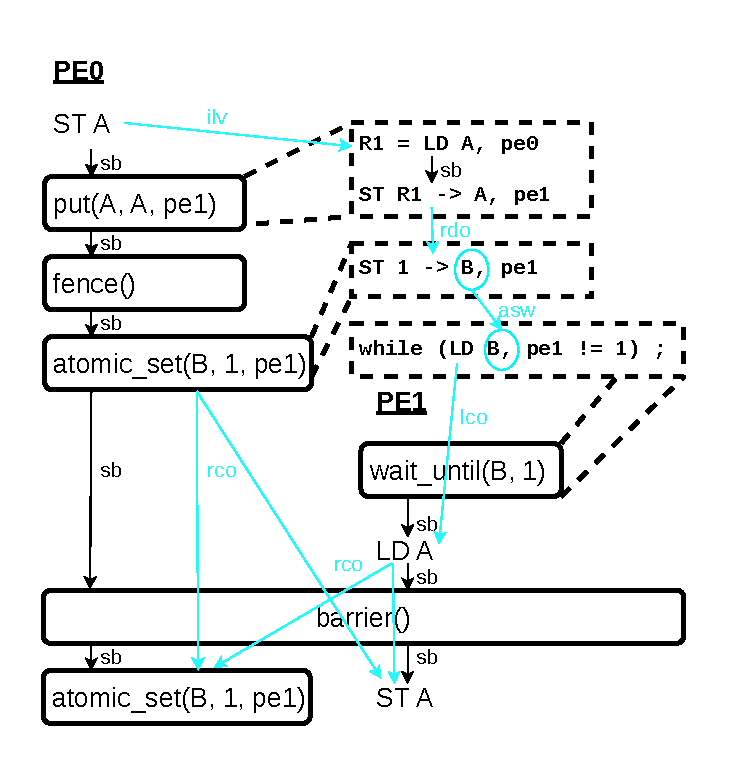
\includegraphics[width=0.75\textwidth]{figures/api_relations}
\centering
\caption{Example \openshmem code execution depicting observable accesses, example
    API-level relations, and a coalesced barrier collective operation event.}
\label{fig:api_execution}
\end{figure}

Figure~\ref{fig:api_execution} illustrates how the above concepts are applied in an
    example \openshmem code execution. \openshmem operations are denoted by rounded
    boxes, and their observable accesses are shown in dotted square boxes.
Matched barrier calls from each \ac{PE} are coalesced into a single operation event.
Operations are ordered within the calling thread by \relSB{}, but their observable
    accesses are constrained only by the added API relations, described below (in
    addition to \relSB{} orderings within the operation):
\begin{itemize}
\item \relILV{} orders the write of $a$ in PE0 (and all prior \relHB{}-ordered accesses)
    with the read of $a$ from the \PUT{} operation.
\item \relLCO{} orders the read of $a$ in PE1 (and all subsequent hb-ordered accesses)
    with the read of $b$ from the (blocking) \FUNC{wait\_until} operation.
\item \relRDO{} orders the bulk write of $a$ from the \PUT{} operation in PE0 with the
    write of $b$ from the fence-separated \FUNC{atomic\_set} operation.
\item \relRCO{} orders all \relHB{} ordered accesses and the accesses of \relHB{}
    ordered \openshmem operations before and after the coalesced barrier event spanning
    PE0 and PE1.
\item \relASW{} orders the write of $b$ from the \FUNC{atomic\_set} operation in PE0
    with the consuming (\relRF{} related) read of $b$ from the \FUNC{wait\_until}
    operation in PE1.
\end{itemize}
Note that~\ref{fig:api_execution} depicts only a representative sample of API relations,
    since an exhaustive depiction would be cluttered.

\subsubsection{Updating the PL-Level Model to an API-Level Model}\label{subsubsec:api_integrate}

We leverage the newly defined observable accesses and ordering relations to define the
    API-level memory model, which is based on the C11 model summarized in
    Section~\ref{subsubsec:api_pl_baseline}.
We first define a new relation, \relAHB{} (\REL{api\_hb}), to be the transitive closure
    of the C11 \relHB{} and all API-level ordering relations introduced in
    Section~\ref{subsubsec:api_relations}:

\begin{itemize}
    \item $api\_hb := (hb \cup ilv \cup lco \cup rdo \cup rco \cup asw)^+$
\end{itemize}

OpenSHMEM \ac{AMO} operations do not provide mutual atomicity with language-level atomic
    operations. Concurrent accesses to the same location by an \openshmem \ac{AMO} and a
    language-level atomic operation must be ordered by \relAHB{}; otherwise, they
    constitute an API data race and the behavior is undefined. This is consistent with
    the atomicity restrictions in Section~\ref{subsec:amo_guarantees}.

In addition, an \relADR{} is defined to relate any two accesses $A$ and $B$ where all of
    the following are true:
\begin{itemize}
    \item $A$ and $B$ access the same memory location on the same \ac{PE}.
    \item At least one access is a modifying access (write or read-modify-write).
    \item Both $A$ and $B$ are ordinary accesses and at least one of them is not atomic;
        or both are observable memory accesses issued by \openshmem operations and at
        least one is issued by a non-synchronizing \openshmem operation (defined in
        Section~\ref{subsubsec:api_relations}); or one is an ordinary access and the
        other is an observable access issued by an \openshmem operation.
    \item $A$ and $B$ are not related by \relAHB{}.
\end{itemize}

The following axioms are updated to use \relAHB{} rather than \relHB{}. The API-level
    model also requires \openshmem \ac{AMO}s to satisfy read-modify-write atomicity,
    subject to the atomicity-domain and datatype restrictions in
    Section~\ref{subsec:amo_guarantees}:
\begin{itemize}
    \item $acyclic(api\_hb)$: \relAHB{} cannot have any cycles.
    \item $irreflexive(rf;api\_hb)$: \relAHB{} must be consistent with the \relRF{}
        relation.
    \item $irreflexive((rf^{-1})^{?};mo;rf^?;api\_hb)$: \relAHB{} must be consistent
        with \relMO{} between writes, and it must also be consistent with the order of
        reads that read from writes in \relMO{} (often called coherence requirement).
    \item $irreflexive(rf \cup (mo;mo;rf^{-1}) \cup (mo;rf))$: The read of an atomic
        read-modify-write access must always read the last value (in \relMO{}) written
        before the write of the read-modify-write access (often called RMW atomicity).
    \item $irreflexive(rf;sb^{amo\_op} \cup (mo;mo;(sb^{amo\_op})^{-1};rf^{-1}) \cup
        (sb^{amo\_op};mo;rf))$: The observable read of an \openshmem \ac{AMO} must
        always read the last value (in \relMO{}) written before the observable write of
        the \ac{AMO} (the \ac{AMO} analog of the PL-level RMW atomicity axiom). Here,
        $sb^{amo\_op}$ is the $sb$ relation between the observable read and write
        accesses issued by an \ac{AMO}.
\end{itemize}

Finally, similar to the C11 memory model, if an \relADR{} exists in a candidate
    execution that satisfies the above axioms, then the behavior is undefined. If an
    \relADR{} does not exist, then the behavior must conform to one of the
    axiom-satisfying candidate executions.

\subsubsection{Compatibility with a Scoped Memory Model}\label{subsubsec:api_scoped}

Accelerator programming models often extend CPU-oriented memory models with
    synchronization scopes. A scope applies to an atomic access and identifies the group
    of threads with which that access may synchronize. In a scoped memory model,
    synchronizing accesses must use a scope that includes both participating threads;
    otherwise, the execution may be a heterogeneous data race under that model.

The \openshmem API does not expose synchronization scopes. An implementation may use
    appropriately scoped synchronization internally, for example when a nonblocking
    operation is performed by a helper thread. Such implementation-internal
    synchronization must be transparent to the user and must not require the user to
    know the locations of implementation helper threads. The API-level guarantees remain
    portable across implementations, whether or not their underlying memory models use
    scopes.
